%tecnologiasprevias
\section{Tecnologías Previas}
\subsection{Código de barras unidimensional}

El código de barras unidimensional (1D) o lineal, pertenecen a la información al variar el ancho y el espaciado de la lineas paralelas en blanco y negro. \cite{2012_Betances}

 
Son los códigos con rayas que se encuentran en la mayoría de los productos de consumo. Estos códigos de barra, permiten a los usuarios de teléfonos móviles acceder a información relacionada a través de Internet, sin necesidad de escribir el nombre del producto.\cite{Reischach2010}

Todo lo que cuenta es qué tan anchos y en qué orden se colocan las barras verticales y los espacios, no importa que tan altos o cortos sean. Se denominan como unidimensionales porque la información contenida en ellos se comunican solo por su dimensión horizontal (consisten en una serie de barras verticales y de espacios) y su posición de izquierda a derecha.
Así como, para automatizar el proceso de identificación de artículos se colocaron los códigos de producto universal (UPC), estos se encuentran en las etiquetas de precios y paquetes de productos en una tienda, supermercados y otros lugares. Evitando así, escribir manualmente el nombre del producto, se puede escanear fácilmente una entrada de datos. Esto aumenta la automatización y reduce el error humano. \cite{2012_DENSO,2012_Varallyai}

\begin{figure} 
\centering
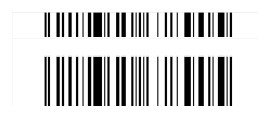
\includegraphics[width=0.5\linewidth]{1Dbarcodes.jpg}
\caption{Cambiar la altura de las barras no cambia la información que contienen}
\label{fig:1dbarcodes}
\end{figure}
\begin{figure} 
\centering
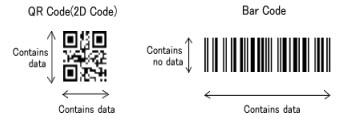
\includegraphics[width=0.5\linewidth]{QRvsBarcode.jpg}
\caption{El código QR (izquierda) contiene información tanto horizontal como vertical, mientras el código de barra (derecha) solo horizontal.}
\label{fig:barcode}
\end{figure}

